\documentclass[]{article}
\usepackage{lmodern}
\usepackage{amssymb,amsmath}
\usepackage{ifxetex,ifluatex}
\usepackage{fixltx2e} % provides \textsubscript
\ifnum 0\ifxetex 1\fi\ifluatex 1\fi=0 % if pdftex
  \usepackage[T1]{fontenc}
  \usepackage[utf8]{inputenc}
\else % if luatex or xelatex
  \ifxetex
    \usepackage{mathspec}
  \else
    \usepackage{fontspec}
  \fi
  \defaultfontfeatures{Ligatures=TeX,Scale=MatchLowercase}
\fi
% use upquote if available, for straight quotes in verbatim environments
\IfFileExists{upquote.sty}{\usepackage{upquote}}{}
% use microtype if available
\IfFileExists{microtype.sty}{%
\usepackage{microtype}
\UseMicrotypeSet[protrusion]{basicmath} % disable protrusion for tt fonts
}{}
\usepackage[margin=1in]{geometry}
\usepackage{hyperref}
\PassOptionsToPackage{usenames,dvipsnames}{color} % color is loaded by hyperref
\hypersetup{unicode=true,
            pdftitle={The geometry and ecology of curved flowers and their pollinators},
            colorlinks=true,
            linkcolor=blue,
            citecolor=blue,
            urlcolor=blue,
            breaklinks=true}
\urlstyle{same}  % don't use monospace font for urls
\usepackage{graphicx,grffile}
\makeatletter
\def\maxwidth{\ifdim\Gin@nat@width>\linewidth\linewidth\else\Gin@nat@width\fi}
\def\maxheight{\ifdim\Gin@nat@height>\textheight\textheight\else\Gin@nat@height\fi}
\makeatother
% Scale images if necessary, so that they will not overflow the page
% margins by default, and it is still possible to overwrite the defaults
% using explicit options in \includegraphics[width, height, ...]{}
\setkeys{Gin}{width=\maxwidth,height=\maxheight,keepaspectratio}
\IfFileExists{parskip.sty}{%
\usepackage{parskip}
}{% else
\setlength{\parindent}{0pt}
\setlength{\parskip}{6pt plus 2pt minus 1pt}
}
\setlength{\emergencystretch}{3em}  % prevent overfull lines
\providecommand{\tightlist}{%
  \setlength{\itemsep}{0pt}\setlength{\parskip}{0pt}}
\setcounter{secnumdepth}{0}
% Redefines (sub)paragraphs to behave more like sections
\ifx\paragraph\undefined\else
\let\oldparagraph\paragraph
\renewcommand{\paragraph}[1]{\oldparagraph{#1}\mbox{}}
\fi
\ifx\subparagraph\undefined\else
\let\oldsubparagraph\subparagraph
\renewcommand{\subparagraph}[1]{\oldsubparagraph{#1}\mbox{}}
\fi

%%% Use protect on footnotes to avoid problems with footnotes in titles
\let\rmarkdownfootnote\footnote%
\def\footnote{\protect\rmarkdownfootnote}

%%% Change title format to be more compact
\usepackage{titling}

% Create subtitle command for use in maketitle
\providecommand{\subtitle}[1]{
  \posttitle{
    \begin{center}\large#1\end{center}
    }
}

\setlength{\droptitle}{-2em}

  \title{The geometry and ecology of curved flowers and their pollinators}
    \pretitle{\vspace{\droptitle}\centering\huge}
  \posttitle{\par}
    \author{}
    \preauthor{}\postauthor{}
    \date{}
    \predate{}\postdate{}
  

\begin{document}
\maketitle

\hypertarget{what-is-curvature}{%
\paragraph{3. What is curvature?}\label{what-is-curvature}}

Reviewing the literature leads us to ask, ``what is curvature?''.
Turning to the field of geometry, we find several related definitions,
resulting from a history of independent mathematical derivations
(reviewed in Coolidge, \protect\hyperlink{ref-coolidge_1952}{1952};
Bardini and Gianella, \protect\hyperlink{ref-bardini_2016}{2016}). Here,
we follow the conventions of Casey
(\protect\hyperlink{ref-casey_1996}{1996}) and Rutter
(\protect\hyperlink{ref-rutter_2000}{2000}), and present a definition
relevant to the problem of analyzing biological shapes.

Intuitively, when a line deviates from being straight we say it is
curved, the extent to which it is not straight is its curvature. More
technically, a line deviates from being straight when its first
derivative - the tangent (shown by \(T_0\), \(T_2\), \(T_n\) in
\href{Figure_3.jpg}{Figure 3}) - changes direction (e.g.~the difference
in direction of \(T_i\) to \(T_{i+1}\). Therefore, curvature can be
thought of as the rate of change in the tangent as we move across the
curve. Hence, the tangent of a straight line has the same direction
everywhere and a curvature of zero, whereas the tangents of the curve
shown in \href{Figure_3.jpg}{Figure 3} will have a non-zero curvature.

To formalize these concepts mathematically we begin by considering an
ordinary function of the form \(y=f(x)\), where \(f(x)\) specifies one
value of \(y\) for each value of \(x\). Biological curves, however,
often loop back on themselves (e.g.~spirals) and are better described by
parametric fuctions that allow the curve to have multiple \(y\) values
for a single \(x\). Parametric functions use a `hidden' variable that
determines the values of \(x\) and \(y\) independently. For example, we
use the parameter arc length, \(s\), along the curve. The position
\((x_i, y_i)\) is solely determined by the corresponding arc length,
\(s_i\), along the curve. We define the location along the curve by a
vector \(\mathbf{\bar{r}}\), which is a function of arc length \(s\):

\begin{equation}
\tag{1}

r_i =
\mathbf{\bar{r}}(s_i) \equiv \left[\begin{array}
{rrr}
x(s_i) \\
y(s_i) \\
\end{array}\right]

\end{equation}

Where \(\mathbf{\bar{r}}(s_i)\) indicates that our position
\(r_i = (x_i, y_i)\) on the curve is determined by the length of the
segment \(s_i\). Although we could parameterize a curve by any arbitrary
variable, arc length is a convienient parameter because it allows us to
move along the curve at even increments of \(\Delta s\). This proves
useful when taking repeated, equally-spaced measurements along a curve,
such as curvature.

If we are interested in the derivative properties of our arc-length
parameterized function, we can differentiate \(\mathbf{\bar{r}}(s)\)
with respect to arc length \(s\) as:

\begin{equation}
\tag{2}

\lim\limits_{\Delta s \to 0} \frac{\Delta \mathbf{\bar{r}}}{\Delta s} = \frac{d \mathbf{\bar{r}}}{ds} = T  

\end{equation}

The resultant tangent function \(T = \frac{d \mathbf{\bar{r}}}{ds}\) is
the first derivative of the parametric equation \(\mathbf{\bar{r}}(s)\).
The tangent \(T_i\) contains information about the direction of the
curve at position \(\mathbf{\bar{r}}(s_i)\) that we will use to
calculate curvature.

At the beginning of this section we defined curvature (\(\kappa\)) as
the rate at which the tangent is changing direction. We can now
formalize this by differentiating \(T\) with respect to arc length:

\begin{equation}
\tag{3}

\kappa = \frac{dT}{ds}

\end{equation}

Where \(\frac{dT}{ds}\) is the second derivative of the parameteric
function \(\mathbf{\bar{r}}(s_i)\):

\begin{equation}
\tag{4}

\kappa_n = \lim\limits_{\Delta s \to 0} \frac{T_{n+ \Delta s} - T_{n- \Delta s}}{2 \Delta s} = \frac{dT_n}{ds_n}

\end{equation}

When the tangent is placed into a cartesian plane its direction is
related to the angle \(\phi\) formed with the \(x\)-axis. We can then
re-state curvature at a single point as:

\begin{equation}
\tag{5}

\kappa = \frac{d\phi}{ds}

\end{equation}

This definition provides an intuitive unit of measurement for reporting
curvature: degrees of rotation per unit arc length
\href{Figure_4.jpg}{(Figure 4)}. For example, if arc length has been
measured in millimeters, we would report its curvature as degrees per
millimeter \(\phi \cdot mm^{-1}\). Framed this way curvature is a
measurement of rotation per distance. In previous defintions (reviewed
in the preceeding section) curvature is an indivisble, single property
of an entire shape. Here, curvature is a property of every point along
the curve. Consequently, we can summarize the \emph{total curvature}
(Milnor, \protect\hyperlink{ref-milnor_1954}{1954}) of a specimen. To do
this, we sum the individual curvature measurements made along the curve.
This is calculated as:

\begin{equation}
\tag{6}

\kappa_{total} = \int_{0}^{s} \kappa \; ds 

\end{equation}

Units for \emph{total curvature} are no longer expressed as
\(\phi \cdot mm^{-1}\) because we are not measuring curvature at a
single point. Instead we are summarizing all tangent rotations along the
curve, expressed simply as \(\phi\).

To account for size variation between specimens, we propose using
\emph{total adjusted curvature}, that is, total curvature divided by arc
length:

\begin{equation}
\tag{7}

\kappa_{adj} = \frac{\kappa_{total}}{s} 

\end{equation}

Units for \(\kappa_{adj}\) are expressed as \(\phi \cdot mm^{-1}\).
\emph{Total adjusted curvature} also represents mean curvature of the
curve.

\begin{figure}
\centering
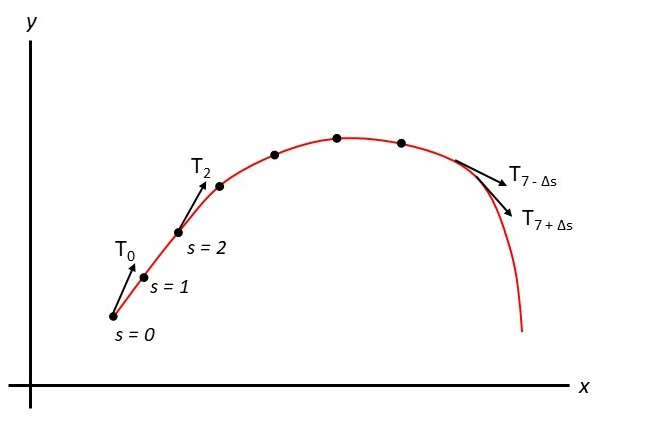
\includegraphics{Figures/Figure_3.jpg}
\caption{Figure 3. A curve parameterized by arc length (\(s\)). When
\(s=5\), the vector \(\mathbf{\bar{r}}(s_5)\) points to the location on
the curve \((x_5, y_5)\). \(T_0\), \(T_2\), and \(T_5\) are the tangents
( \(\frac{d \mathbf{\bar{r}}}{ds}\) ) at \(s=0\), \(s=2\), and \(s=5\),
respectively. Curvature at \(s_n\) is defined in equation (4).}
\end{figure}

\hypertarget{a-proposed-protocol-for-measuring-curvature}{%
\paragraph{4. A proposed protocol for measuring
curvature}\label{a-proposed-protocol-for-measuring-curvature}}

As illustrated in the methodology review, our current protocols for
measuring flower-pollinator curvature lack a conceptual unity. In each
method, curvature takes on a new meaning. Therefore, there are two main
advantages of the curvature definition described above. First, curvature
becomes a local property of the tissue or organ under study. This means
that shape information is gathered at every point along the curve and
can be examined and compared to other points within or between
specimens. This differs from previous methods that take curvature as a
total property of the entire curve. In these measurements curvature
cannot be parsed into smaller elements. Second, because the revised
definition is explicitly adapted from the field of differential
geometry, we benefit from citeable geometric concepts that allow us to
be clear about what we mean by `curvature'.

In order to apply the above definition of curvature, a biological organ
or tissue needs to be reduced to a continuous function. We propose a
workflow as illustrated in \href{Figures/Figure_4.jpg}{Figure 4}.
Cosgrove (\protect\hyperlink{ref-cosgrove_1990}{1990}) uses an analogous
approach to study the development of cucumber hypocotyls. By fitting
cubic splines to hand-marked seedlings, curvature was computed using the
same definition as above. However, since Cosgrove
(\protect\hyperlink{ref-cosgrove_1990}{1990}), the entire field of
landmark-based geometric morphometrics has unfolded (reviewed in Adams
et al., \protect\hyperlink{ref-adams_2013}{2013}). This rigorous,
reproducible toolkit has been used extensively in pollination ecology,
but has not yet been leveraged to calculate curvature
(\href{Tables/Table_1.csv}{Table 1}). Terral et al
(\protect\hyperlink{ref-terral_2004}{2004}) use these tools to digitally
landmark olive stones and fit polynomials to the landmarks: synthesizing
the concepts of Cosgrove (\protect\hyperlink{ref-cosgrove_1990}{1990})
and Terral (\protect\hyperlink{ref-terral_2004}{2004}) produces a
modernized method for fitting curves and computing curvature from
biological forms \href{Figures/Figure_4.jpg}{(Figure 4)}

\begin{figure}
\centering
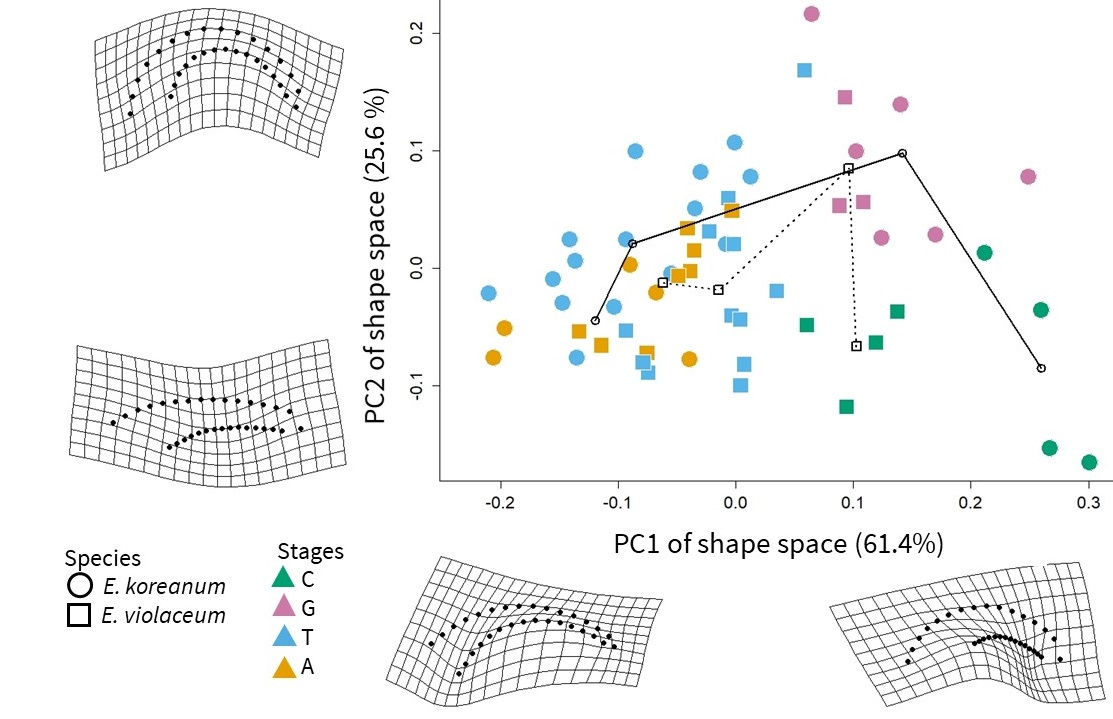
\includegraphics{Figures/Figure_4.jpg}
\caption{Figure 4: Proposed protocol for measuring curvature. 1. A petal
of \emph{Epimedium violaceum} is landmarked and rotated. 2. A polynomial
curve is fitted to the landmarks. 3. Curvature is calculated as the rate
of change of the tangent vector at every point along the curve. Total
curvature can be calculated by the methods outlined in Section 3.}
\end{figure}

Comment on why using we're using polynomials and not splines, fourier,
etc.

\hypertarget{refs}{}
\leavevmode\hypertarget{ref-adams_2013}{}%
Adams, D.C., Rohlf, F.J., and Slice, D.E. (2013). A field comes of age:
Geometric morphometrics in the 21st century. Hystrix \emph{24}, 7.

\leavevmode\hypertarget{ref-bardini_2016}{}%
Bardini, G., and Gianella, G.M. (2016). A historical walk along the idea
of curvature, from Newton to Gauss passing from Euler. International
Mathematical Forum \emph{11}, 259--278.

\leavevmode\hypertarget{ref-casey_1996}{}%
Casey, J. (1996). Exploring curvature (Braunschweig, Germany: Friedr.
Vieweg \& Sohn Verlagsgesellschaft mbH).

\leavevmode\hypertarget{ref-coolidge_1952}{}%
Coolidge, J.L. (1952). The unsatisfactory story of curvature. The
American Mathematical Monthly \emph{59}, 375--379.

\leavevmode\hypertarget{ref-cosgrove_1990}{}%
Cosgrove, D.J. (1990). Rapid, bilateral changes in growth rate and
curvature during gravitropism of cucumber hypocotyls: Implications for
mechanism of growth control. Plant, Cell \& Environment \emph{13},
227--234.

\leavevmode\hypertarget{ref-milnor_1954}{}%
Milnor, J. (1954). On total curvatures of closed space curves.
Mathematica Scandinavica \emph{1}, 289--296.

\leavevmode\hypertarget{ref-rutter_2000}{}%
Rutter, J.W. (2000). Geometry of curves (Boca Raton, FL: CRC Press,
Taylor; Francis Group).

\leavevmode\hypertarget{ref-terral_2004}{}%
Terral, J.-F., Alonso, N., Capdevila, R.B. i, Chatti, N., Fabre, L.,
Fiorentino, G., Marinval, P., Jordá, G.P., Pradat, B., Rovira, N., et
al. (2004). Historical biogeography of olive domestication (olea
europaea l.) as revealed by geometrical morphometry applied to
biological and archaeological material. Journal of Biogeography
\emph{31}, 63--77.


\end{document}
